%!TEX root = karen.tex

\chapter{Keeneland Benchmarks}
\label{app:keeneland_alltoallv_benchmarks}

This appendix provides new data from Keeneland, a supercomputing cluster designed with 240 six-core Intel Xeon 5660 (2.80GHz) CPUs with HyperThreading (HT) enabled (x2 threads per core), 12MB cache per core shared on chip, 24GB system memory, and 360 NVidia M2070 GPUs with 6GB of device memory and 14 multiprocessors each \cite{Vetter2011}.  A high level layout of the Keeneland system is presented in Figure~\ref{fig:keeneland}. The system was designed with its 240 CPUs partitioned into sets of two CPUs per compute node, four nodes per chassis, and six chassis per rack. An InfiniBand QDR Network handles inter-node communication. In addition to the dual CPUs, each node has three NVidia M2070 Fermi class GPUs.

\begin{figure}
\centering
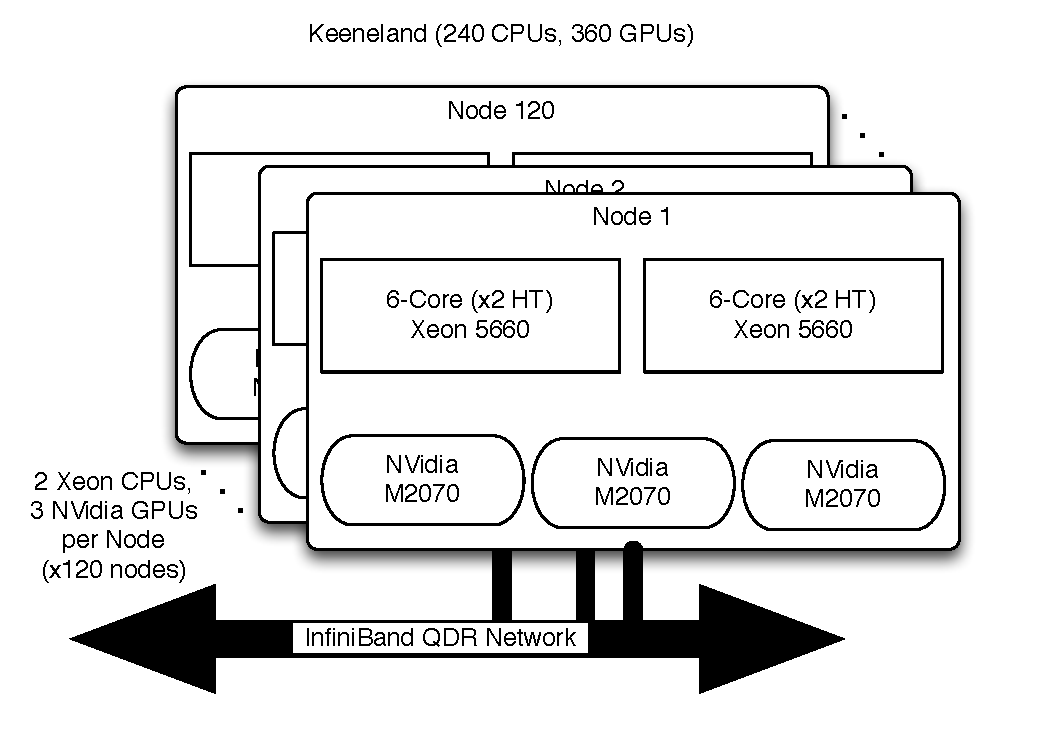
\includegraphics[width=0.5\textwidth]{../figures/omnigraffle/Keeneland.pdf}
\caption{The Keeneland Initial Delivery System (KIDS), a multi-GPU cluster with 360 GPUs and 240 CPUs capable of 201 TFLOP/sec.}
\label{fig:keeneland}
\end{figure}

At the onset of this dissertation, the KID system provided the initial development environment for our multi-CPU and multi-GPU implementation. In Spring 2012, the KID system was upgraded to the Keeneland Full Scale (KFS) system and the M2070 GPUs (150 Gbyte/sec bandwidth) were replaced by M2090 GPUs (177 Gbyte/sec \cite{M2090}). 

All data in this Appendix was acquired prior to the 2012 upgrade and is provided for direct comparison with our first paper (\cite{BolligFlyerErlebacher2012}), which demonstrated scaling of the test cases in \S~\ref{sec:cosine_bell} and \S~\ref{sec:vortex_rollup}. The distributed RK4 iteration utilized the primitive MPI\_Send/MPI\_Recv communication routines to simulate a round-robin, all-to-subset collective where each processor took a turn to send data (0 or more bytes) or otherwise waited to receive messages. The choice of blocking routines were useful for code verification. 

The implementation demonstrated poor scaling behavior as blocking collectives serialized transmissions, and every processor had to wait until the end of the collective to proceed. A linear-in-$x$ partitioning was also employed on the sphere, which only worsens scaling (as shown in Section~\ref{sec:load_balance}). However, the objective in \cite{BolligFlyerErlebacher2012}, was not to present a well tuned implementation of RBF-FD for distributed GPU environments. Rather, we focused on the design decisions for partitioning, index mapping, etc. and verification of both single and distributed GPU implementations---as inefficient as they were. 

The benchmarks provided here replace the serialized sends and receives with an MPI\_Alltoallv. Communication times have dropped significantly and improved scaling of the implementation. The linear partitioning remains, although the effects of the imbalanced workloads are not apparent because benchmarks only scale up to 10 GPUs with one process (i.e., one GPU) per node. All benchmarks on the GPU measure runtime of the custom OpenCL kernels described in Section~\ref{sec:custom_gpu_kernels}.  

Unfortunately, shortly after the transition from KIDs to KFS our research allocation expired leaving scaling benchmarks for greater than 10 GPUs untested. The tuning efforts in Chapters~\ref{chap:distributed_rbffd} and \ref{chap:multigpu_rbffd} that provided load balancing and added overlapping communication and computation were completed too late to test on Keeneland. 


\section{Single GPU Performance} 

In \cite{BolligFlyerErlebacher2012} only speedup plots are provided to demonstrate improvement by the GPU over the CPU. For better analysis, data is presented here in both GFLOP/sec and speedup form. 

Consider the performance of a full RK4 iteration for the Cosine Bell Advection test case in \S~\ref{sec:cosine_bell}. As discussed in Chapter~\ref{chap:gpu_rbffd}, a regular SpMV involves $(2Nn)$ FLOPs. Intermediate evaluations in the RK4 time-step (i.e., the steps $k_{1 ... 4}$ in Equation~\ref{eqn:rk4}) perform three SpMV operations: one for each $D_{\theta}$, $D_{\lambda}$ and $D_{hv}$, plus another seven vector operations to scale and join derivatives ($5N$) and prep the input for the subsequent evaluation ($2N$). The cost of evaluating an intermediate step is therefore estimated at $(6Nn + 7N)$ FLOPs. In that case, the four evaluations of an RK4 Cosine Bell iteration, plus an additional $5N$ FLOPs overhead to combine intermediate solutions totals to: $(24Nn + 33N)$ FLOPs. 

The Vortex Roll-Up from \S~\ref{sec:cosine_bell} computes only two SpMVs per intermediate evaluation of the RK4 time-step for a cost of $(4Nn + 5N)$. Following the same logic for the RK4 iteration we arrive at the total estimate: $(16Nn + 25N)$ FLOPs. 

Using the FLOP estimate for each case, Figure~\ref{fig:gflops_cpu_1proc_keeneland} provides the average GFLOP/sec observed for a single time-step of Cosine Bell Advection (Figure~\ref{fig:gflops_cpu_1proc_keeneland_cosine}) and Vortex Roll-Up (Figure~\ref{fig:gflops_cpu_1proc_keeneland_vortex}) on a single CPU in Keeneland. The average time is calculated over 10000 time-steps. In both cases the CPU performs the SpMV operation by running a simple nested loop on data packed in CSR format. The Intel compiler applies auto-vectorization, auto-blocking and other strategies to the nested loop based on the ``-O2" compiler flag. 


\begin{figure}
\centering
\begin{subfigure}[t]{0.425\textwidth}
\centering
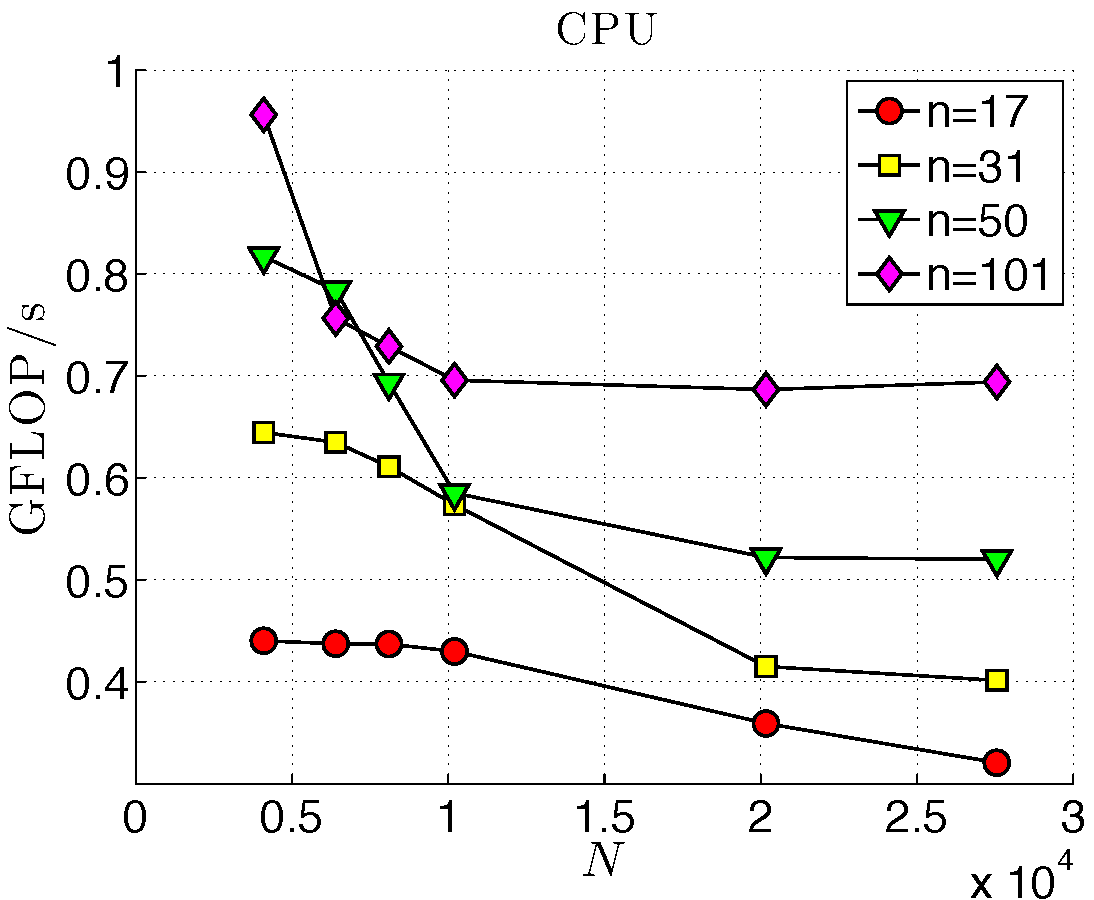
\includegraphics[width=\textwidth]{../figures/keeneland_results/alltoallv_cosine/gflops_cpu_1proc_oneWarpPerStencil.pdf}
%\end{subfigure}
\caption{Cosine Bell Advection}
\label{fig:gflops_cpu_1proc_keeneland_cosine}
\end{subfigure} 
\quad
\begin{subfigure}[t]{0.425\textwidth}
\centering
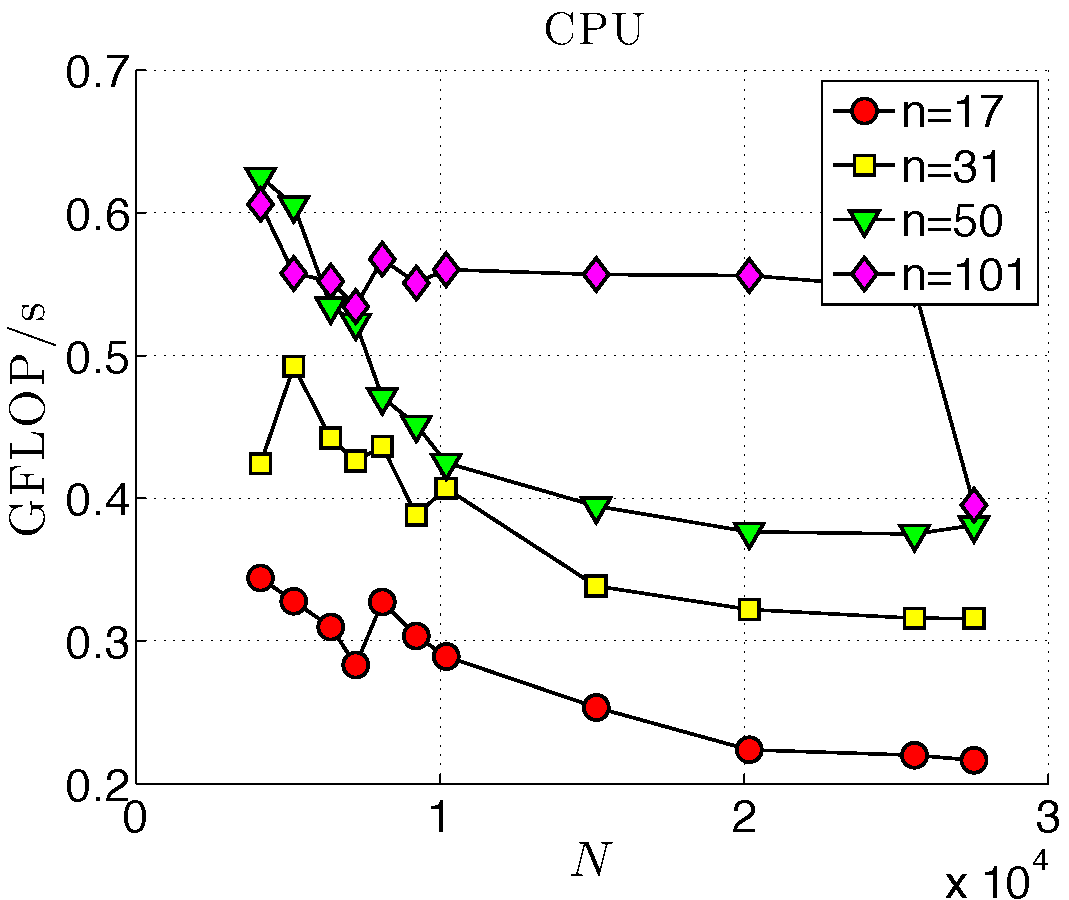
\includegraphics[width=\textwidth]{../figures/keeneland_results/alltoallv_vortex/gflops_cpu_1proc_oneWarpPerStencil.pdf}
\caption{Vortex Roll-Up}
\label{fig:gflops_cpu_1proc_keeneland_vortex}
\end{subfigure}
\caption{GFLOP/sec on one CPU (1 core) of the Keeneland GPU cluster.}
\label{fig:gflops_cpu_1proc_keeneland}
\end{figure}

Figure~\ref{fig:gflops_gpu_1proc_oneWarp_keeneland_cosine} and \ref{fig:gflops_gpu_1proc_oneWarp_keeneland_vortex} show the GFLOP/sec achieved by operating one warp per stencil in our custom GPU kernels on the M2070 GPUs. Once again the data is packed in a CSR format. The corresponding speedups achieved over the CPU is provided in Figures~\ref{fig:speedup_1proc_oneWarp_keeneland_cosine} and \ref{fig:speedup_1proc_oneWarp_keeneland_vortex}. Due to its higher operation count, the Cosine Bell Advection is able to achieve over 2.75 GFLOP/sec for $n=101$, nearly double the Vortex Roll-Up case. Also, by operating as warps dedicated to each stencil, the OpenCL kernel nicely maintains a consistent GFLOP/sec in all cases. 

%TODO: warp allows us to predict performance of stencil size

\begin{figure}
\centering
\begin{subfigure}[t]{0.46\textwidth}
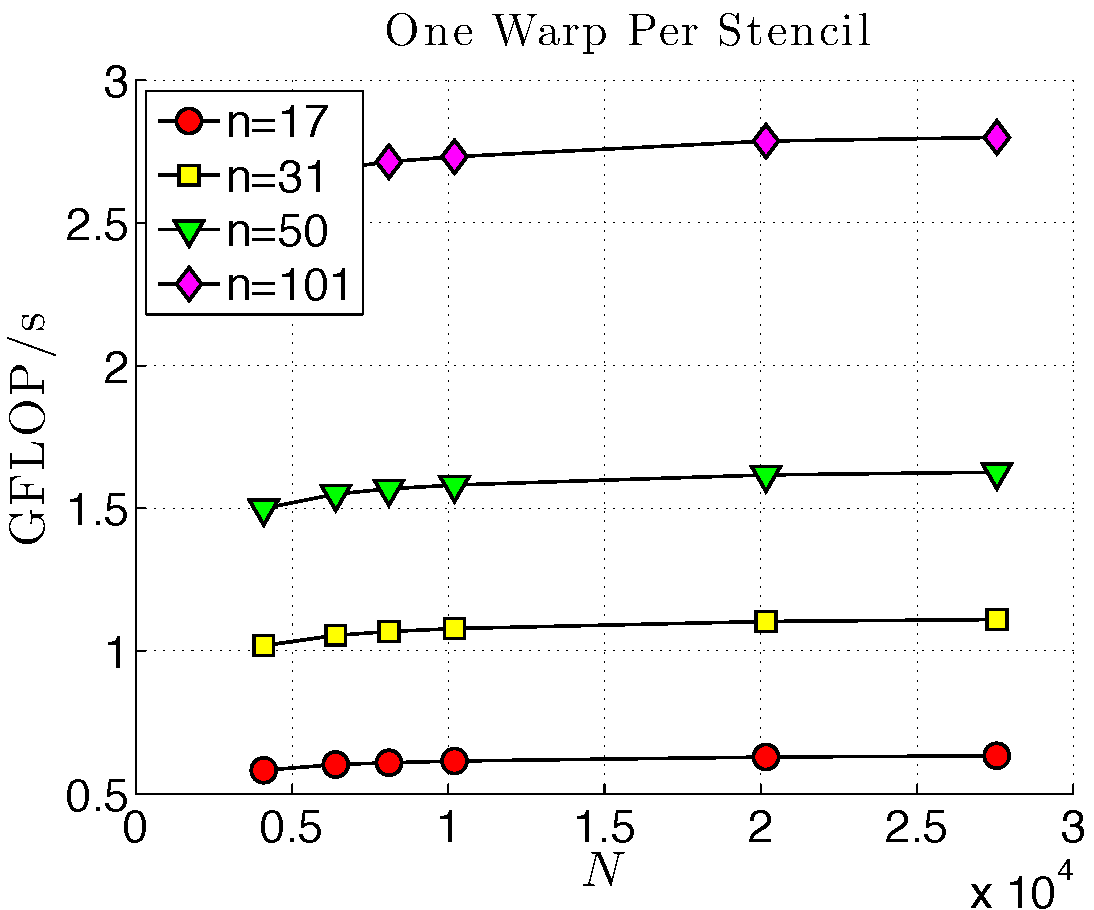
\includegraphics[width=\textwidth]{../figures/keeneland_results/alltoallv_cosine/gflops_gpu_1proc_oneWarpPerStencil.pdf}
\caption{GFLOP/sec (Cosine Bell).}
\label{fig:gflops_gpu_1proc_oneWarp_keeneland_cosine}
\end{subfigure} 
\quad
\begin{subfigure}[t]{0.425\textwidth}
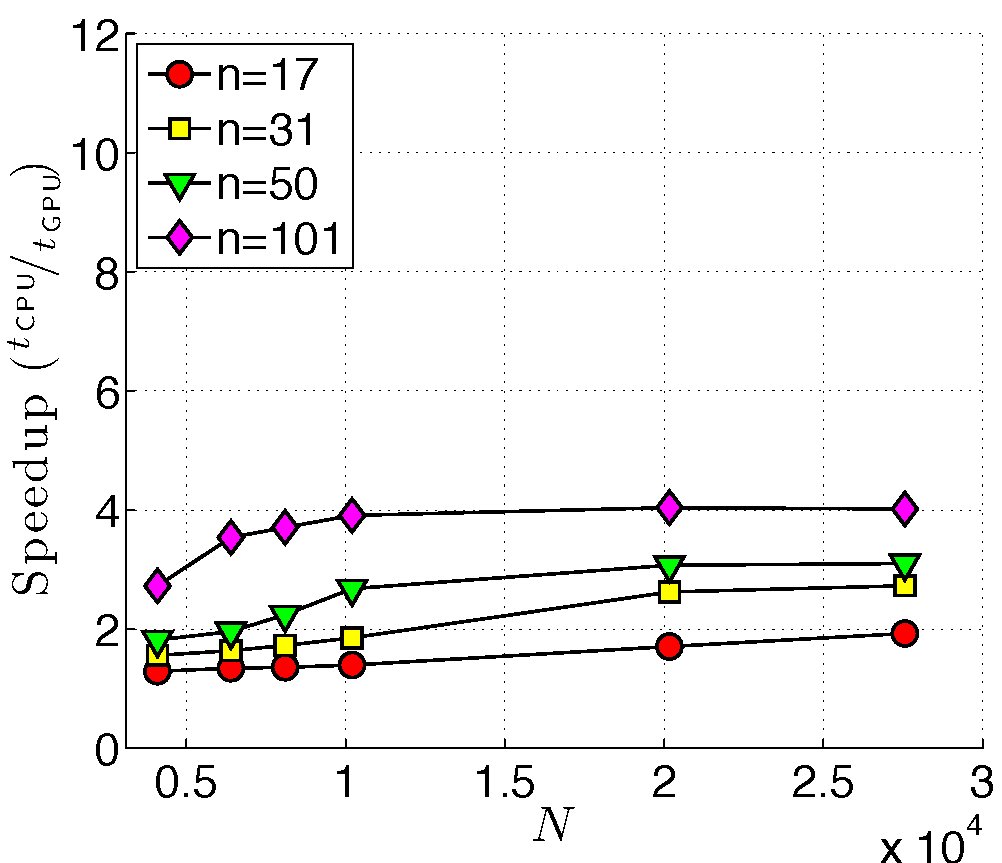
\includegraphics[width=\textwidth]{../figures/keeneland_results/alltoallv_cosine/speedup_1proc_oneWarpPerStencil.pdf}
\caption{Speedup versus one CPU (Cosine Bell).}
\label{fig:speedup_1proc_oneWarp_keeneland_cosine}
\end{subfigure} 

\begin{subfigure}[t]{0.46\textwidth}
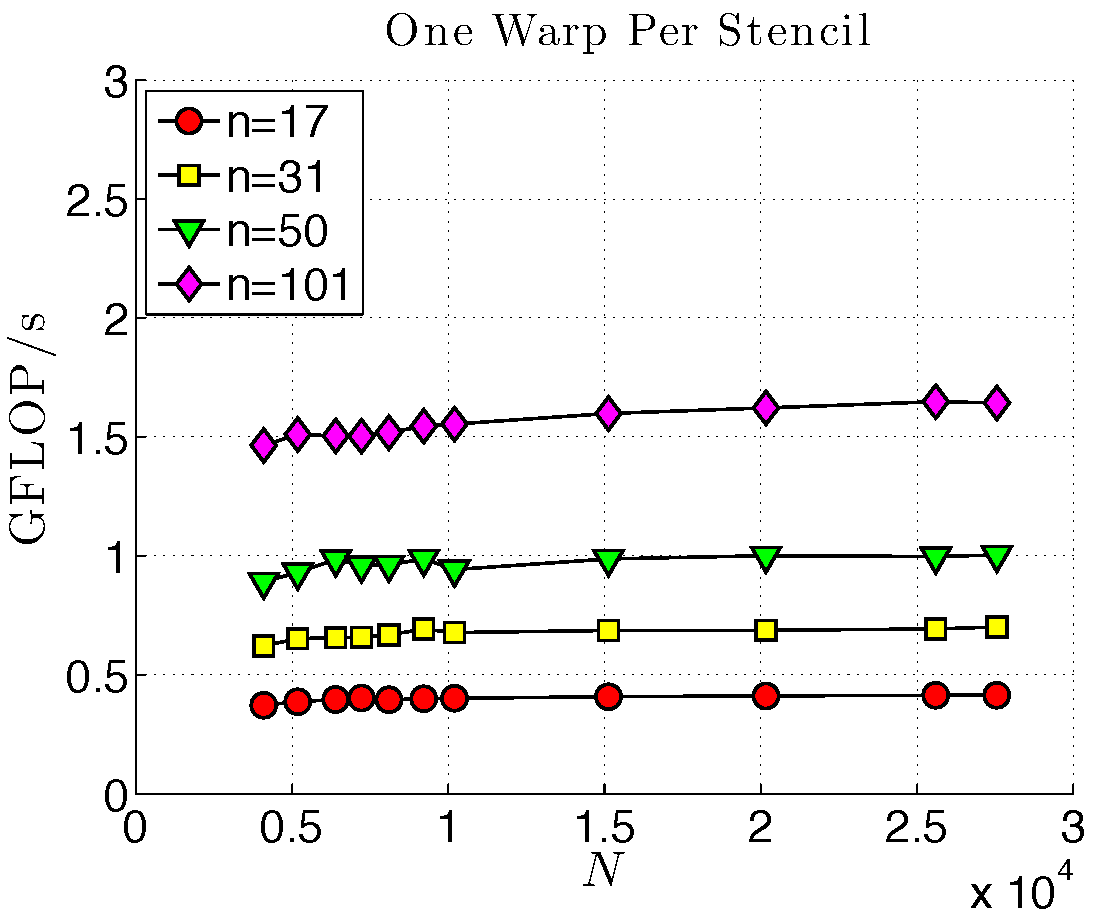
\includegraphics[width=\textwidth]{../figures/keeneland_results/alltoallv_vortex/gflops_gpu_1proc_oneWarpPerStencil.pdf}
\caption{GFLOP/sec (Vortex Roll-Up)}
\label{fig:gflops_gpu_1proc_oneWarp_keeneland_vortex}
\end{subfigure} 
\quad
\begin{subfigure}[t]{0.425\textwidth}
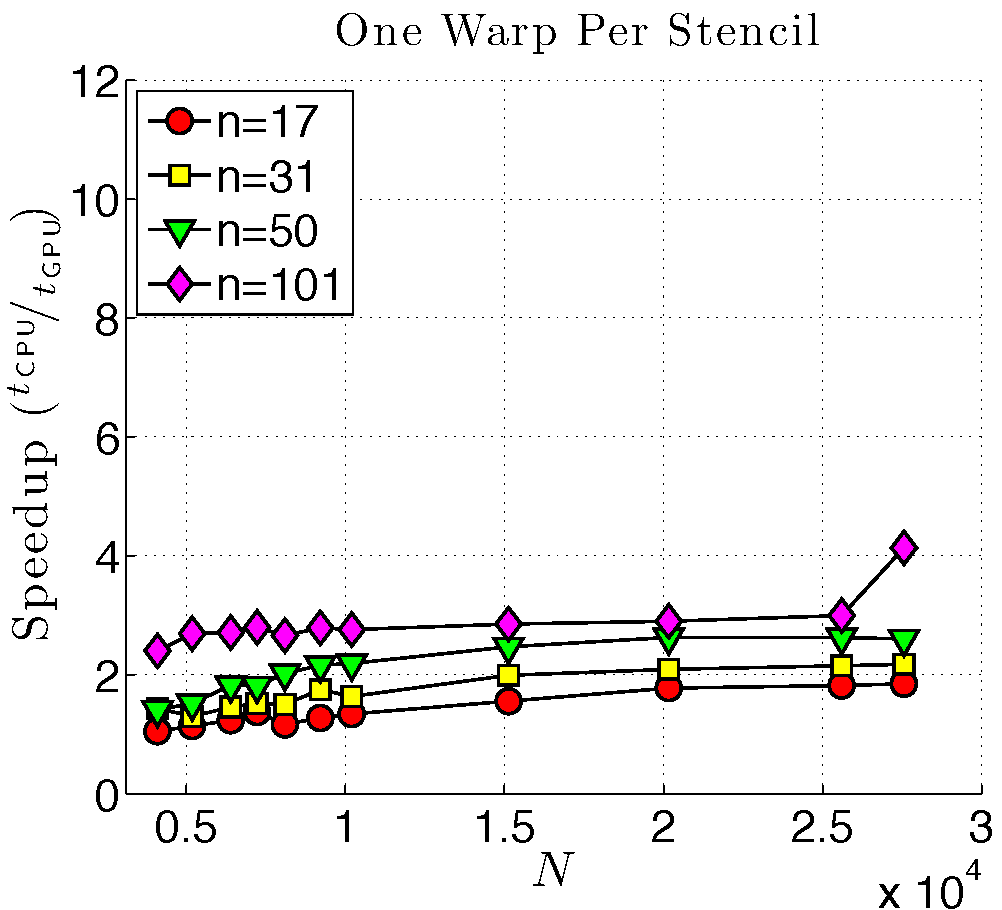
\includegraphics[width=\textwidth]{../figures/keeneland_results/alltoallv_vortex/speedup_1proc_oneWarpPerStencil.pdf}
\caption{Speedup versus one CPU (Vortex Roll-Up)}
\label{fig:speedup_1proc_oneWarp_keeneland_vortex}
\end{subfigure} 
\caption{GFLOP/sec and Speedup observed on one GPU (M2070) of the Keeneland GPU cluster for Cosine Bell Advection and Vortex Roll-Up when operating by ``One Warp Per Stencil" within the RK4 kernel.}
\label{fig:1proc_oneWarp_keeneland}
\end{figure} 

In similar fashion the GFLOP/sec achieved by operating one thread per stencil is demonstrated in Figure~\ref{fig:gflops_gpu_1proc_oneWarp_keeneland_cosine} (Cosine Bell) and \ref{fig:gflops_gpu_1proc_oneThread_keeneland_vortex} (Vortex Roll-Up). Speedups over the CPU for the thread approach are given in Figures~\ref{fig:speedup_1proc_oneThread_keeneland_cosine} and \ref{fig:speedup_1proc_oneThread_keeneland_cosine}. 


\begin{figure}
\centering
\begin{subfigure}[t]{0.46\textwidth}
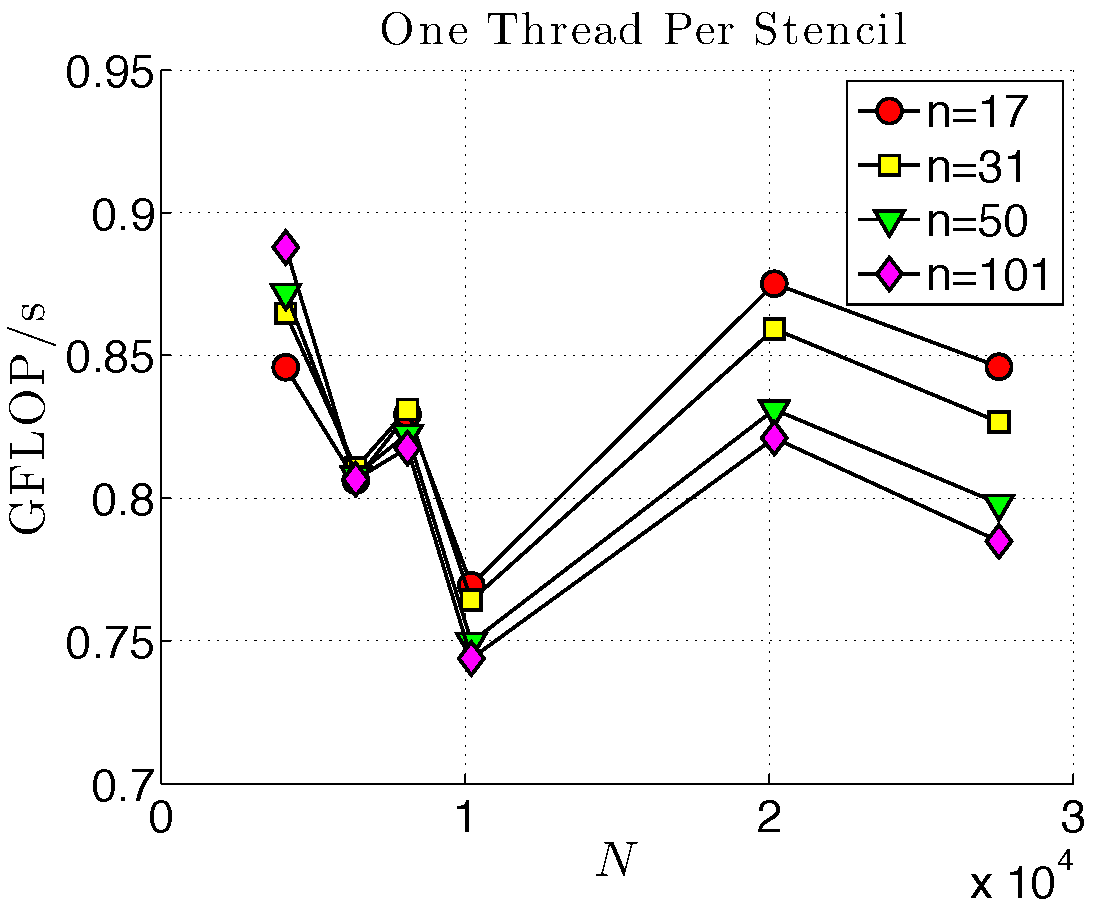
\includegraphics[width=\textwidth]{../figures/keeneland_results/alltoallv_cosine/gflops_gpu_1proc_oneThreadPerStencil.pdf}
\caption{GFLOP/sec (Cosine Bell).}
\label{fig:gflops_gpu_1proc_oneThread_keeneland_cosine}
\end{subfigure}
\quad
\begin{subfigure}[t]{0.425\textwidth}
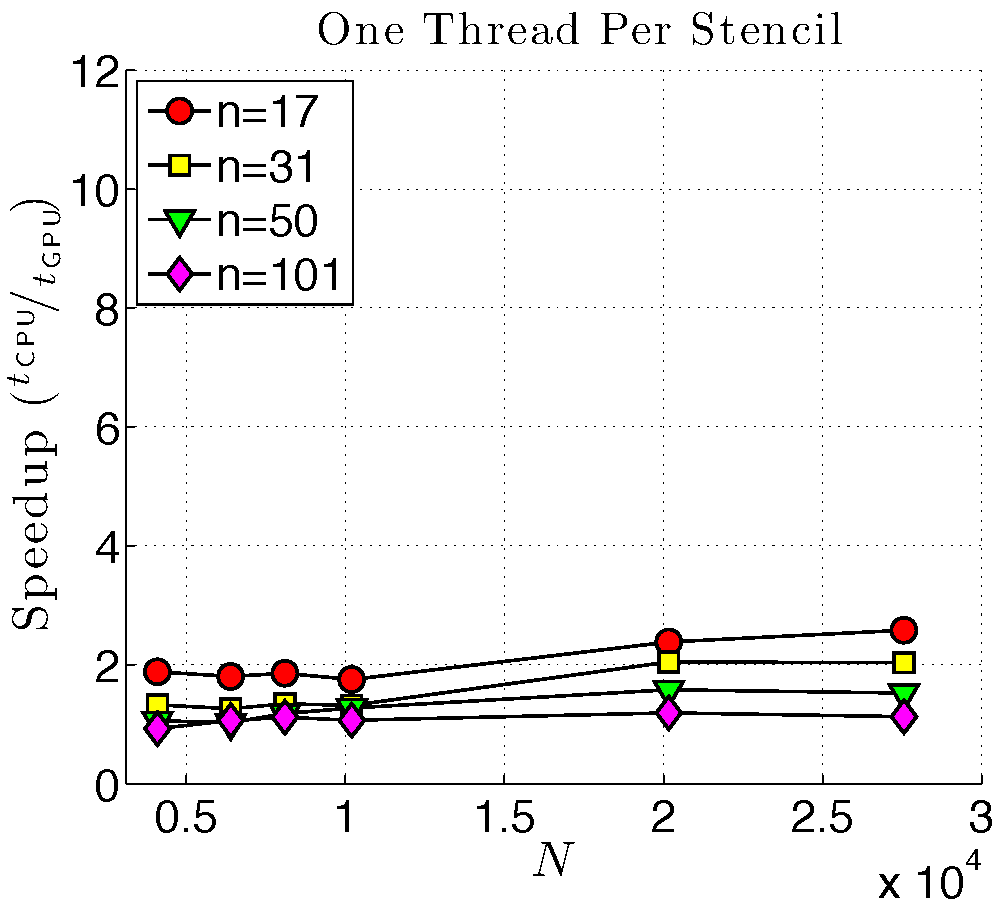
\includegraphics[width=\textwidth]{../figures/keeneland_results/alltoallv_cosine/speedup_1proc_oneThreadPerStencil.pdf}
\caption{Speedup (Cosine Bell).}
\label{fig:speedup_1proc_oneThread_keeneland_cosine}
\end{subfigure} 

\begin{subfigure}[t]{0.46\textwidth}
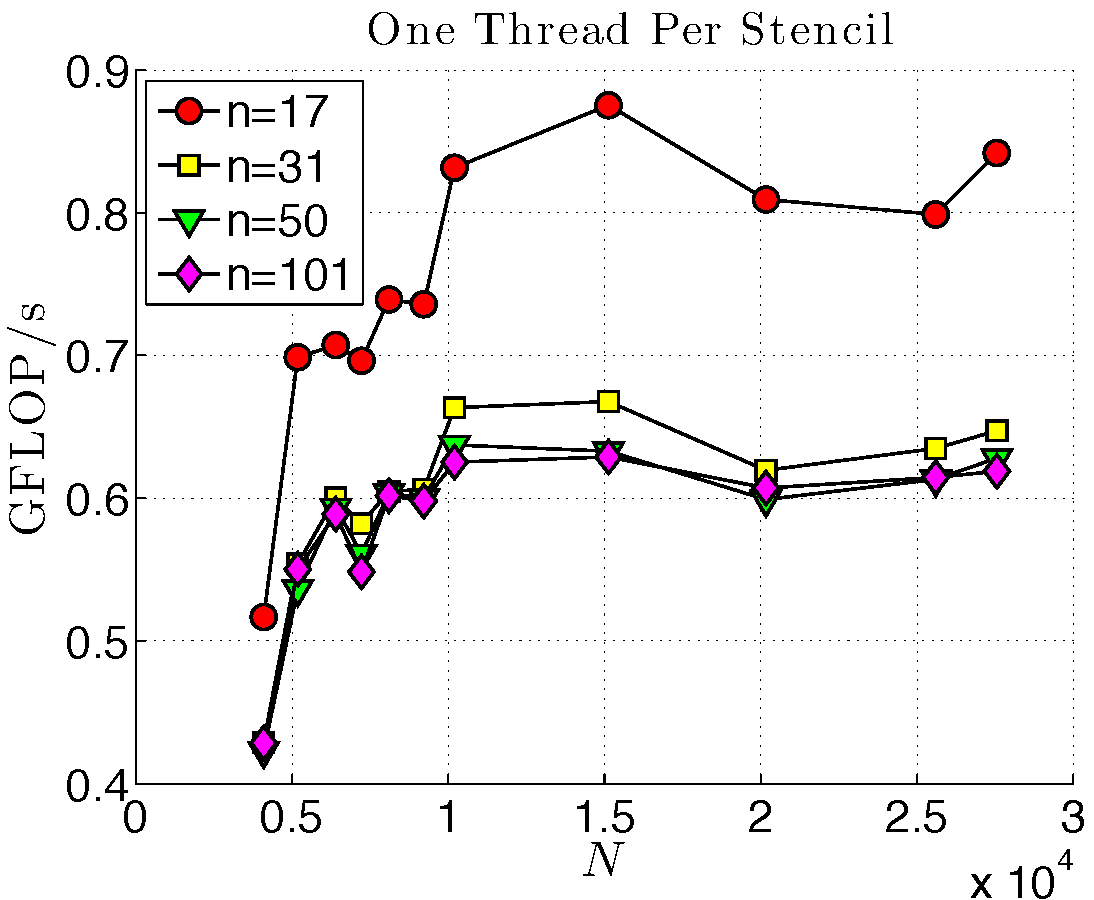
\includegraphics[width=\textwidth]{../figures/keeneland_results/alltoallv_vortex/gflops_gpu_1proc_oneThreadPerStencil.pdf}
\caption{GFLOP/sec (Vortex Roll-Up)}
\label{fig:gflops_gpu_1proc_oneThread_keeneland_vortex}
\end{subfigure}
\quad
\begin{subfigure}[t]{0.425\textwidth}
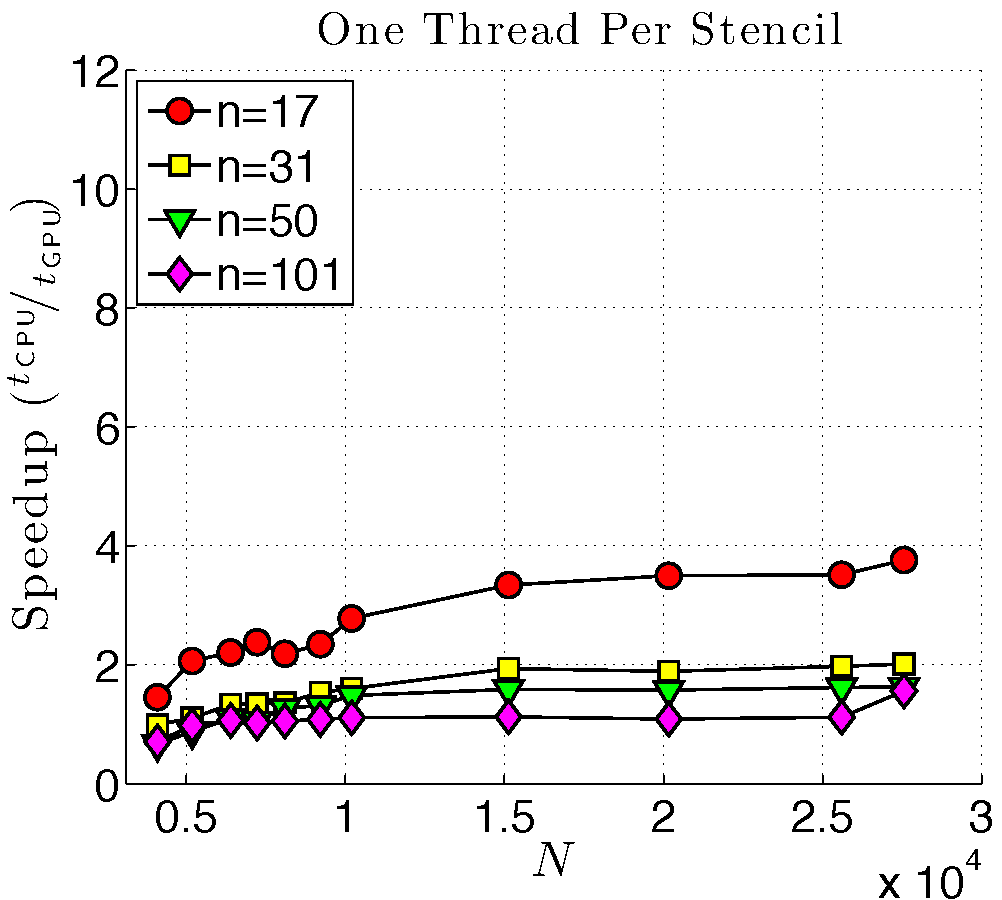
\includegraphics[width=\textwidth]{../figures/keeneland_results/alltoallv_vortex/speedup_1proc_oneThreadPerStencil.pdf}
\caption{Speedup (Vortex Roll-Up)}
\label{fig:speedup_1proc_oneThread_keeneland}
\end{subfigure} 
\caption{GFLOP/sec and Speedup observed on one GPU (M2070) of the Keeneland GPU cluster when operating by ``One Thread Per Stencil" within the RK4 kernel.}
\label{fig:1proc_oneThread_keeneland}
\end{figure} 

Based on data in Figures~\ref{fig:1proc_oneWarp_keeneland} and \ref{fig:1proc_oneThread_keeneland} we observe: 
\begin{enumerate} 
\item For stencils of size $n < 32$, operating with perfect concurrency across stencils (i.e., operating one thread per stencil) allows for the highest GFLOP/sec by stencil size. Unfortunately, this approach achieves nearly equivalent GFLOP/sec across all stencil sizes, which emphasizes its limited applicability and diminishing returns. The achieved GFLOP/sec is also less predictable than the warp counterpart. 
\item Operating by warp has surprisingly predictable performance. Each curve grows slightly as $N$ scales, but the most significant factor impacting GFLOP/sec is the stencil size.
\item The additional operations for the third SpMV in cosine bell advection (Figure~\ref{fig:speedup_1proc_oneWarp_keeneland_cosine}) also contribute significantly to the achieved throughput. This is to be expected as the RBF-FD (SpMV) is a memory bound problem, and the GPU work-items sit idle waiting for data to reach them. The added complexity of another SpMV makes use of cached data for the vector and is easily computed long before the idle time finishes. 
\end{enumerate}
These observations lead to the conclusion, that although operating one thread per stencil is an option, under most circumstances operating by a warp on stencils is preferred. We also note that the demonstrated performance of the ELL matrix format in Chapter~\ref{chap:gpu_rbffd} is far superior to the data shown here. As such, effort to further tune these two kernels was diverted to continuing investigations with the help of the ViennaCL ELL matrix. 


\section{Keeneland Scaling with MPI\_Alltoallv}

The following data demonstrates performance of the implementation with an MPI\_alltoallv collective. These benchmarks consider the cosine bell advection from Section~\ref{sec:cosine_bell}. 

Figure~\ref{fig:alltoall_multicpu_scaling} shows the strong scalability of our method on multiple CPUs. This figure demonstrates that our method does scale linearly (almost super-linearly) as the number of CPUs increases. 
%, so our prospect for spanning all CPUs on Keeneland is within reach for problem sizes large enough.
The super-linear speedup is due to improved caching on processors as individual problem sizes decrease and the processors are able to keep a larger percentage of the problem within fast cache memory.

\begin{figure}
\centering
\begin{subfigure}[t]{0.425\textwidth}
\centering
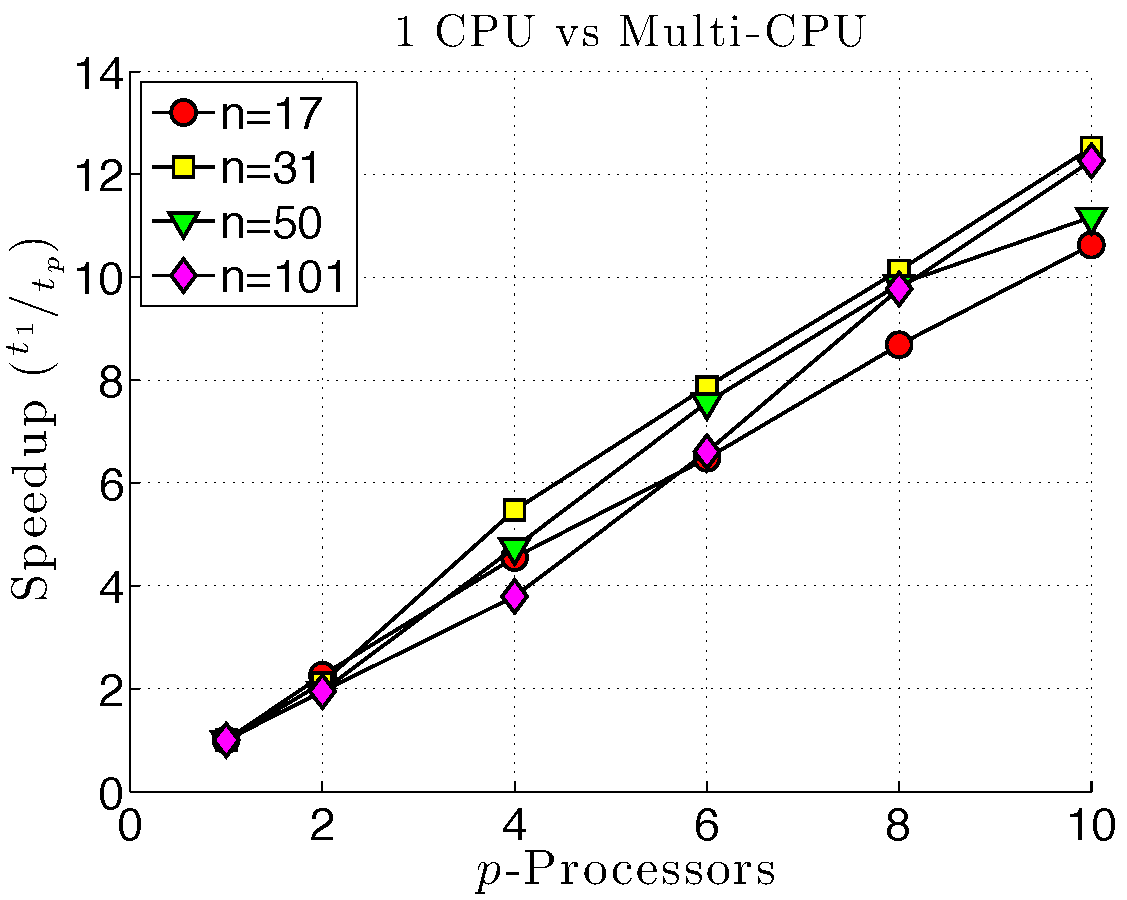
\includegraphics[width=1.0\textwidth]{../figures/keeneland_results/alltoallv_cosine/speedup_1CPU_vs_NCPU.pdf}
\caption{Multi-CPU strong scaling. The problem size is sufficiently large to hide latency in MPI communication.}
\label{fig:alltoall_multicpu_scaling}
\end{subfigure} 
\begin{subfigure}[t]{0.425\textwidth}
\centering
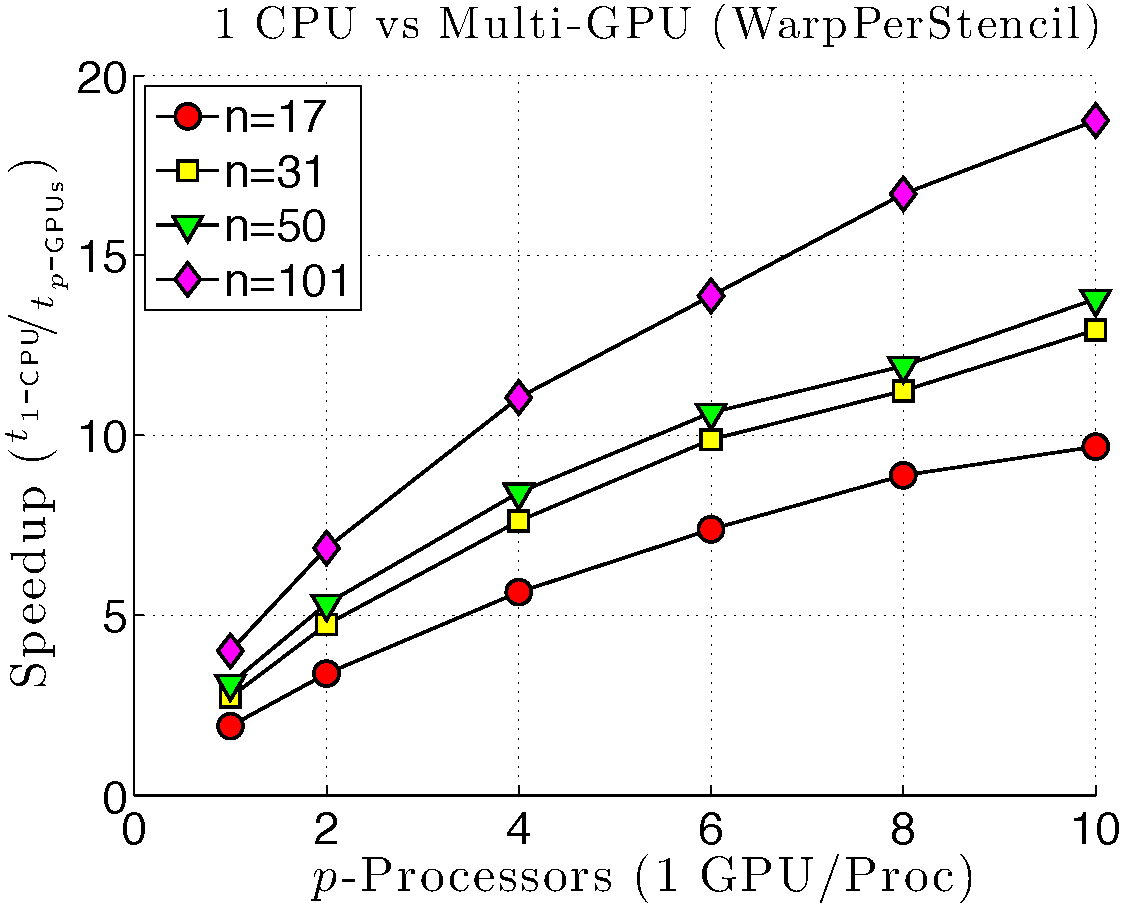
\includegraphics[width=1.0\textwidth]{../figures/keeneland_results/alltoallv_cosine/speedup_1CPU_vs_NGPU_WarpPerStencil.pdf}
\caption{Multi-GPU strong scaling vs one CPU}
\label{fig:alltoall_multigpu_vs_cpu_scaling}
\end{subfigure} 
\begin{subfigure}[t]{0.425\textwidth}
\centering
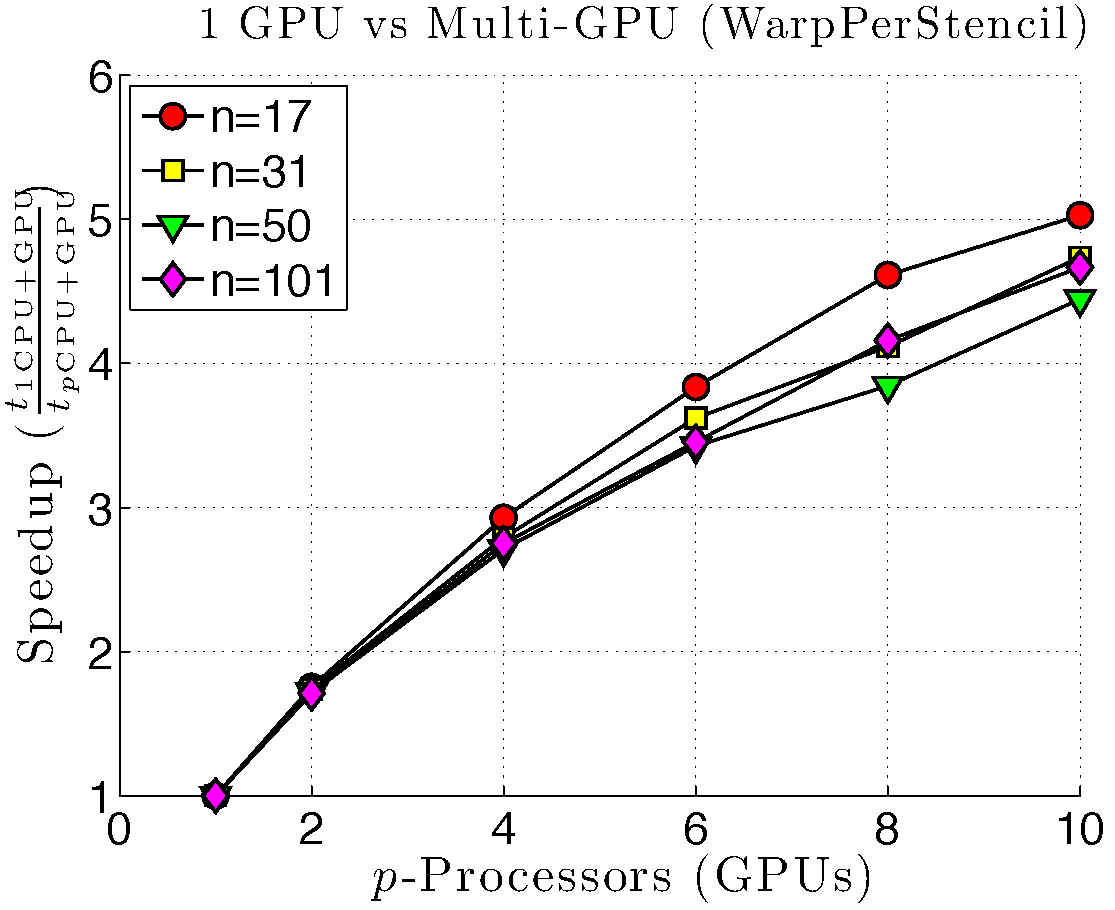
\includegraphics[width=1.0\textwidth]{../figures/keeneland_results/alltoallv_cosine/speedup_1GPU_vs_NGPU_WarpPerStencil.pdf}
\caption{Multi-GPU strong scaling vs one GPU}
\label{fig:alltoall_multigpu_vs_gpu_scaling}
\end{subfigure} 
\caption{Multi-CPU and Multi-GPU strong scaling on Keeneland for the ``One Warp per Stencil" RK4 implementation}
\end{figure}

\begin{figure}
\centering
\begin{subfigure}[t]{0.425\textwidth}
\centering
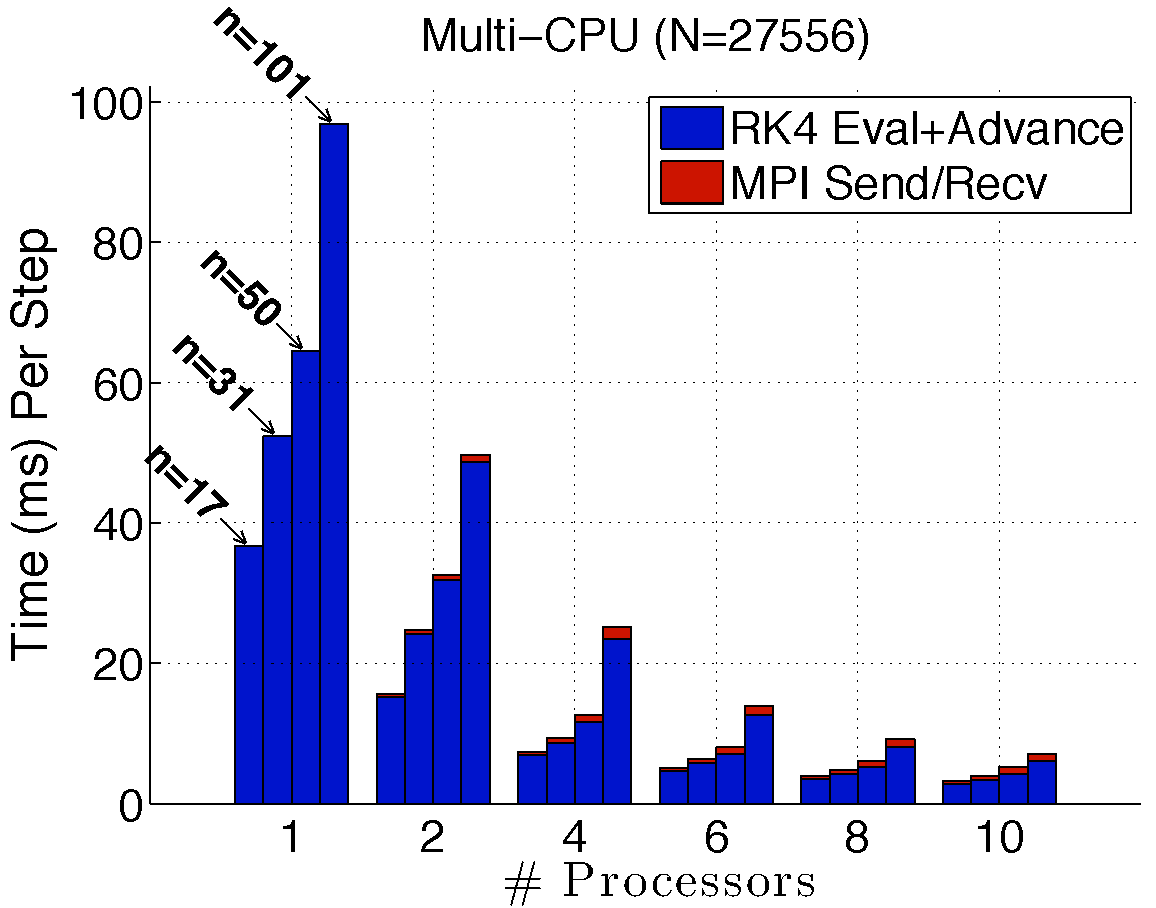
\includegraphics[width=1.0\textwidth]{../figures/keeneland_results/alltoallv_cosine/multiCPU_costs.pdf}
\caption{Multi-CPU}
\label{fig:alltoall_multicpu_costs}
\end{subfigure} 
\begin{subfigure}[t]{0.425\textwidth}
\centering
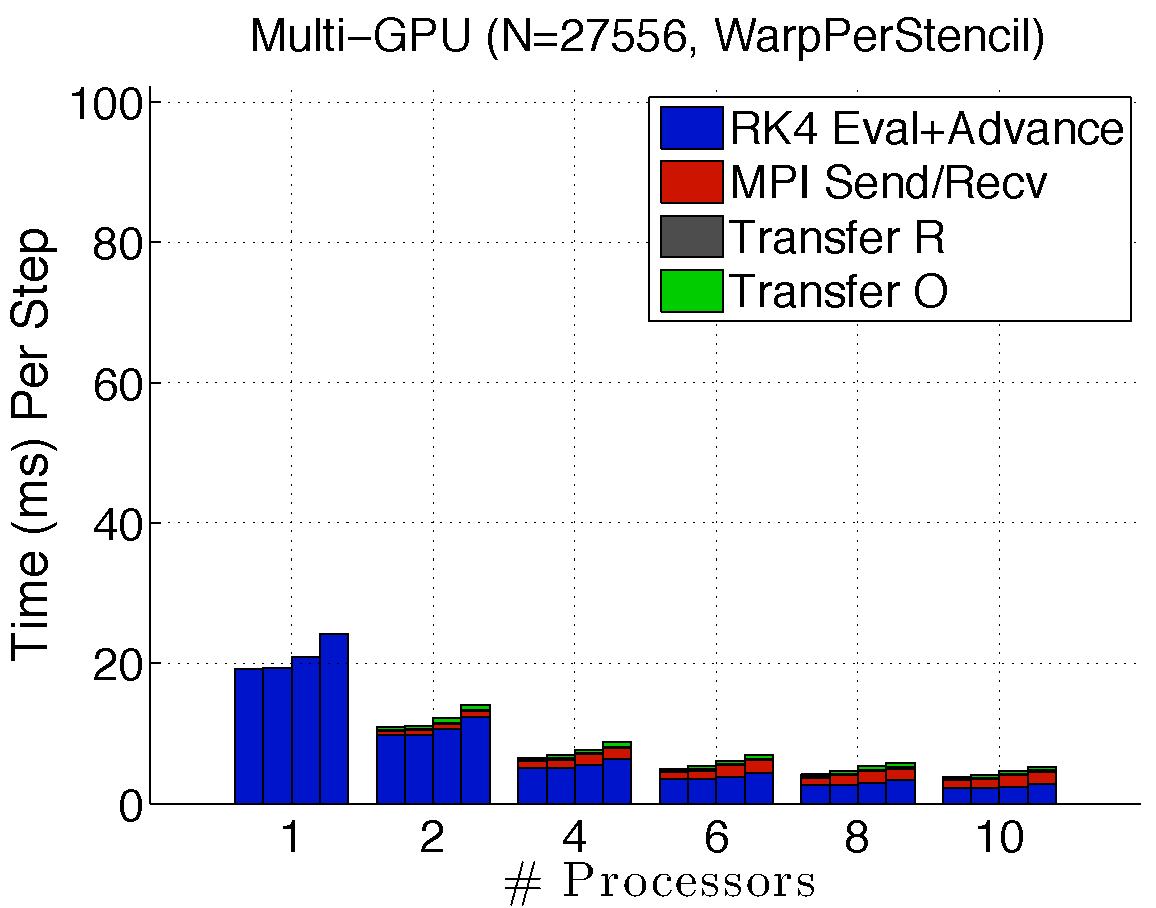
\includegraphics[width=1.0\textwidth]{../figures/keeneland_results/alltoallv_cosine/multiGPU_warp_costs.pdf}
\caption{Multi-GPU}
\label{fig:alltoall_multigpu_costs}
\end{subfigure} 
\caption{Cost comparison of benchmark components on Keeneland. The cost of MPI communication is significantly reduced and allows further scaling. When the GPU accelerates computation, the non-parallelizable time for MPI\_Alltoallv and data transfers between GPU and CPU quickly become the dominant factors.}
\end{figure} 

Figure~\ref{fig:alltoall_multigpu_vs_cpu_scaling}  shows the scaling of multiple GPUs vs 1 CPU. Ideally, this figure would be the product of Figures~\ref{fig:alltoall_multicpu_scaling} and \ref{fig:gflops_gpu_1proc_oneWarp_keeneland_vortex} since the GPUs are attached to CPUs in a one to one correspondence. However, the sub-linear scaling is quickly tapering off. In this case the cost of MPI communication is the same as in the previous figure. Operating on the GPU has two effects: a) the fraction of computation in the iteration is reduced, which means MPI communication dominates faster; and b) the GPU adds the cost of data transfers between host and device further exacerbating the situation. 

Figure~\ref{fig:alltoall_multigpu_vs_gpu_scaling} shows the scalability of multiple GPUs vs 1 GPU. Here we see a sub-linear behavior for all cases. This is attributed to both the cost of transfer between CPUs and GPUs and the decreasing problem size as number of processors increases, which underutilizes the GPUs. 


Figure~\ref{fig:alltoall_multicpu_costs} and Figure~\ref{fig:alltoall_multigpu_costs} show a great reduction in time per iteration dedicated to communication compared to the figures in \cite{BolligFlyerErlebacher2012}. In the Figure~\ref{fig:alltoall_multigpu_costs}, the way the times bottom out indicates the iteration is converged on the minimum time required to launch a GPU kernel, transfer to/from the GPU, and communicate the problem via MPI. To scale to more processors, a larger problem size is absolutely necessary. 

Leveraging the overlapping communication and computation algorithm from Chapter~\ref{chap:multigpu_rbffd} would hide some/all of the cost in communication, but it also reduces the computation time. 



%I am generating another set of figures that demonstrate the scaling when we overlap communication and computation. MPI collectives do not allow overlap, but the asynchronous GPU kernel launches do. Therefore, I expect:
%    - the scaling on multiple CPUs vs 1 CPU to be the same as it is now
%    - the scaling on multiple GPUs vs 1 GPU will improve to linear/super-linear for problem sizes that occupy the hardware longer than the minimum kernel launch time. For N=27556 we might only see linear speedup up to 6 or 8 processors. 
%    - larger problem sizes will still be necessary (I have benchmarks for 100K, 500K and 1M on the sphere).
%    

%TODO: Work-Group Size and Number of Stencils
%What if a work-group is larger than a warp? What if the group was occupied by multiple stencils. What improvements to speedup do we see?
%
%How many stencils can each group handle (assuming values stay in shared memory? 
%Shared memory bank conflicts? How do we sort the values? 
%What is the occupancy of the GPU?
%

